% Template for ICASSP-2018 paper; to be used with:
%          spconf.sty  - ICASSP/ICIP LaTeX style file, and
%          IEEEbib.bst - IEEE bibliography style file.
% --------------------------------------------------------------------------
\documentclass{article}



%% packages
\usepackage{spconf}
% graph
\usepackage{graphicx}
\usepackage{epstopdf}
\usepackage{array}
\usepackage{rotating}
\usepackage{tabularx}
% math
\usepackage{amsfonts}
\usepackage{amsmath}
\usepackage{mathtools}
% algorithm
\usepackage{algorithm,algorithmic}% http://ctan.org/pkg/algorithms

% Example definitions.
% --------------------
\def\x{{\mathbf x}}
\def\L{{\cal L}}

% Title.
% ------
{Tensor-based Discriminative Sensing for Fraud Detection}
%
% Single address.
% ---------------
\name{Thiago P. de B. Vieira and Jo\~ao Paulo C. L. da Costa}
\address{University of Bras\'ilia}

%
% For example:
% ------------
%\address{School\\
%	Department\\
%	Address}
%
% Two addresses (uncomment and modify for two-address case).
% ----------------------------------------------------------
%\twoauthors
%  {A. Author-one, B. Author-two\sthanks{Thanks to XYZ agency for funding.}}
%	{School A-B\\
%	Department A-B\\
%	Address A-B}
%  {C. Author-three, D. Author-four\sthanks{The fourth author performed the work
%	while at ...}}
%	{School C-D\\
%	Department C-D\\
%	Address C-D}
%
\begin{document}
%\ninept
%
\maketitle

\begin{abstract}
The abstract goes here... Compressive Sensing (CS) allows to acquire signals at sampling rates significantly lower than the Nyquist rate, provided that the signals possess a sparse representation in an appropriate basis. However, in some applications of CS, the dictionary providing the sparse description is partially or entirely unknown. It has been shown that dictionary learning algorithms are able to estimate the basis vectors from a set of training samples. In some applications the dictionary is multidimensional, e.g., when estimating jointly azimuth and elevation in a 2-D direction of arrival (DOA) estimation context. In this paper we show that existing dictionary learning algorithms can be extended to exploit this structure, thereby providing a more accurate estimate of the dictionary. As examples we choose two prominent dictionary learning algorithms, the method of optimal directions (MOD) and the K-SVD algorithm. We propose tensor-based multidimensional extensions for both algorithms and show their improved performances numerically.
\end{abstract}

\begin{keywords}
Tensor-Based Dictionary Learning, Fraud Detection, Classification, Unbalanced Data
\end{keywords}

\section{Introduction}
\label{sec:introduction}

Compressive sensing is emergent for signal processing and hás been applied to Fields such as signal restoration, image processing and classification (sparce representation classification src )

Iterative dictionary learning hás been used as a blind technique for feature extraction, improving classification without require feature selection or principal conponent analysis

Big data analytics require techniques to Deal with multidimensional data, making Sense of strucutre and relationship of many dimensios. Pca is commonly adopted for dimensionality reduction and feature extraction. Tensor hás been adopted for multidimensional data analysis and can be explored for dictionary learning

Adaptive techniques for high dimensional and high thoughput

we propose to apply the tensor deconposition for dictionary learning in order to evidentiate the discriminative sensing of a fraud detection dataset

Dictionary Learning is a signal processing technique for sparse representation of signals as basis vectors, learning the representations from training data, as dictionaries. The sparse representation in terms of such dictionaries has attracted increased interest for compressive sensing and for solving problems such as denoising, compression, image processing, data decomposition, feature extraction and classification \cite{tosic2011dictionary, zhang2010discriminative, zhu2016coupled,ravishankar2011mr}.

% There are two major approaches for dictionary learning. First is the analytic approach, in which DCT bases, wavelets, curvelets and other nonadaptive functions are used as atoms to construct the dictionaries. Second is the learning-based approaches, such as the unsupervised learning for dictionary construction [9] and the online dictionary learning [11], [10], which use machine learning methods to construct the dictionary. In the analytic approach, some pre-defined functions are used to construct the dictionary. Curvelets [24], which tracks the shape of the discontinuity set, offers efficient and near-optimal representation of smooth objects. Shearlets [25], which is obtained from dilations, action of translations and shear transformations, has nice geometric properties and mathematical properties for image representation. Bandelets [26], which specifies the geometry as a vector field, is de-signed to improve the image compression and noise reduction performance. In the learning-based approach, machine learning methods are used to construct the dictionary from the training data. The least square error is used by the method of the optimal directions (MOD) [27] to update the dictionary iteratively:
% Dictionaries are either available analytically, or can be learned from a suitable training set. While analytic dictionaries permit to capture the global structure of a signal and allow a fast implementation, learned dictionaries often perform better in applications as they are more adapted to the considered class of signals.

In some applications the data and its dictionary are multidimensional, e.g., when estimating jointly behavior of users in social networks. Computing tensor decompositions of multi-way datasets is particularly useful to extract hidden patterns and structure in multidimensional data analytics problems \cite{kolda2009tensor}. Tensor-based algorithms for dictionary learning can improve the performance for cases of multidimensional and separable data, regarding the dictionary identification rating, the required number of training samples and iterations for the optimization problem \cite{roemer2014tensor}.

% In imagery, the numerical burden for (i) learning a dictionary and for (ii) employing the dictionary for reconstruction tasks only allows to deal with relatively small image patches that only capture local image information. Separable dictionaries aims at overcoming these drawbacks by allowing a separable structure on the dictionary throughout the learning process. On the one hand, this permits larger patch-sizes for the learning phase, on the other hand, the dictionary is applied efficiently in reconstruction tasks. The crucial idea is to allow the dictionary to have a separable structure, where separable means that the dictionary D is given by the Kronecker product of two smaller dictionaries A ∈ R h×a and B ∈ R w×b
% Without loss of generality we choose square image patches with w = h = 8, which is in accordance to the patch-sizes mostly used in the literature

Multidimensional parameter estimation and learning multidimensional separable dictionaries are growing research problems. Roemer \emph{et al.} \cite{roemer2014tensor} show that the multidimensional dictionary estimation problem can be efficiently formulated in terms of tensors, and that their results outperform existing schemes by exploiting the multilinear structure of the problem.

Existing dictionary learning schemes can be applied to multidimensional analysis and obtain valuable results. However, the performance of tensor-based algorithms for recovering of a known separable dictionary outperform existing schemes when dealing with growing multidimensional datasets, as can be seen in Figures \ref{fig:fig1} and \ref{fig:fig2}, which show that the recovering rating of traditional algorithms decreases over the dataset increasing.

\begin{figure}[!htb]
     \centering 
	 \includegraphics[width=0.4\textwidth]{figures/5_20_2000_1000_100.eps}
     \caption{Matrix of 1.000 elements, 2000 sample training, 100 iterations}
     \label{fig:fig1}
\end{figure}

\begin{figure}[!htb]
     \centering 
	 \includegraphics[width=0.4\textwidth]{figures/5_20_2000_24000_100.eps}
     \caption{Matrix of 24.000 elements, 2000 sample training, 100 iterations}
     \label{fig:fig2}
\end{figure}

Figures \ref{fig:fig1} and \ref{fig:fig2} show the evaluation of tensor-based and traditional dictionary learning algorithms for dictionary reconstruction of a multidimensional and separable data. Figure \ref{fig:fig1} presents the results for dictionary reconstruction from a matrix of 1000 elements by 50 atoms, while Figures \ref{fig:fig2} presents the results from a matrix with 24000 entries by 300 atoms. It is possible to observe better reconstruction rating for tensor-based algorithms. 

Imbalanced data...
Recent developments in science and technology have enabled the growth and availability of raw data to occur at an explosive rate. This has created an immense opportunity for knowledge discovery and data engineering research to play an essential role in a wide range of applications from daily civilian life to national security. However, the high availability of raw data increases the challenges related to big data analytics and to imbalanced data, which corresponds to data sets exhibiting significant imbalances of classes or rare events of some classes. The fundamental issue with the imbalanced learning problem is the ability of imbalanced data to significantly compromise the performance of most standard learning algorithms

A key challenge to use sparse coding and dictionary learning for classification is how to find proper dictionaries and coefficients that highligh discriminative structure and relationships of one dataset. Therefore, we introduce a tensor-based dictionary learning method for fraud detecton from unbalanced data. Specifically, we apply a sparse representation based classification (SRC) method through learning a tensor-based dictionary and evaluate the reconstruction error for fraud classification. In this paper, we propose a tensor-based sparse representation and dictionary learning technique to analyze mobile money transactions in order to identify frauds. We propose to use tensor-based dictionary learning for learning fraudulent and legitimante data separetelly, and apply the learned dictionaries to reconstruct a test signal and classify it as fraud or ligitimate, according to the minimum reconstruction error measured by some metrics.

%However, tensor-based algorithms face challenges to achieve reasonable processing time to handle large-scale tensor factorizations \cite{de2014distributed}, demanding efforts in order to explore distributed processing techniques for tensor-based analytics of large datasets. We propose a distributed and tensor-based approach for multidimensional dictionary learning in order to obtain better processing time for larger datasets. We focus on a distributed implementation of T-MOD \cite{roemer2014tensor} algorithm, based on a modification of Almeida and Kibangou's \cite{de2014distributed} approach to use Tucker-2 decomposition. We perform experiments to test different methods for learning dictionaries, evaluating the processing time and the reconstruction of a dictionary of multidimensional and separable data.

\section{Related Works}

Face recognition...

Fisher...

Florian...

Tem que ver outro...

\section{Data Model}

Consider a generic sparse recovery problem of the following form

\begin{equation}\label{eq:eq01}
\boldsymbol{X} = \boldsymbol{A} \cdot \boldsymbol{S} + \boldsymbol{W},
\end{equation}

where $\boldsymbol{X} \in \mathbb{C}^{M \times T}$ represents $T$ consecutive observations from $M$ features, $\boldsymbol{A} \in \mathbb{C}^{M \times N}$ is the overcomplete dictionary, $\boldsymbol{S} \in \mathbb{•}hbb{C}^{N \times T}$ represents the sparse coefficient matrix, $\boldsymbol{W} \in \mathbb{C}^{M \times T}$ is the additive noise, and $M < N < T$.

Consider a sparse recovery problem for a separable 2-D manifold, i.e., a manifold that can be written as the product of two 1-D manifolds. If we choose a separable 2-D sampling grid, we can write the 2D sparse recovery problem as

Imbalance data where zero is predominante

Data divided into learning and test, with isfraud labels with 1 or 0

\begin{equation}\label{eq:eq02}
\boldsymbol{X} = (\boldsymbol{A}^{(1)} \otimes \boldsymbol{A}^{(2)}) \cdot \boldsymbol{S} + \boldsymbol{W},
\end{equation}

where $\boldsymbol{A} = (\boldsymbol{A}^{(1)} \otimes \boldsymbol{A}^{(2)})$, $\boldsymbol{A}^{(1)} \in \mathbb{C}^{M_1 \times N_1}$, $\boldsymbol{A}^{(2)} \in \mathbb{C}^{M_2 \times N_2}$, $M = M_1 \times M_2$, and $N = N_1 \times N_2$.

The Kronecker model (\ref{eq:eq02}) can be rewritten in an equivalent tensor form. Applying the algebraic rules for unfoldings of n-mode products \cite{roemer2014tensor} we can rewrite (\ref{eq:eq02}) into a "Tucker-2" decomposition, as

\begin{equation}\label{eq:eq03}
\boldsymbol{\mathcal{X}} = \boldsymbol{\mathcal{S}} \times_1 \boldsymbol{A}^{(1)} \times_2 \boldsymbol{A}^{(2)} +  \boldsymbol{\mathcal{W}},
\end{equation}

where $\boldsymbol{\mathcal{X}} \in \mathbb{C}^{M_1 \times M_2 \times T}$, $\boldsymbol{\mathcal{S}} \in \mathbb{C}^{N_1 \times N_2 \times T}$, and $\boldsymbol{\mathcal{W}} \in \mathbb{C}^{M_1 \times M_2 \times T}$ are rearranged versions of the matrices $\boldsymbol{X}$, $\boldsymbol{S}$, and $\boldsymbol{W}$ such that $\boldsymbol{X} = [\boldsymbol{\mathcal{X}}]_{(3)}^T$, $\boldsymbol{S} = [\boldsymbol{\mathcal{S}}]_{(3)}^T$, and $\boldsymbol{W} = [\boldsymbol{\mathcal{W}}]_{(3)}^T$, respectively.

We consider a randomly generated data in order to evaluate the proposed approach, where initially $\boldsymbol{A}^{(1)}$ and $\boldsymbol{A}^{(2)}$ are gaussian distributed and randomly generated, then the dictionary $\boldsymbol{A}$ is obtained. In order to be able to evaluate the dictionary reconstruction, the sparse data $\boldsymbol{\mathcal{X}}$ is generated from the dictionary $\boldsymbol{A}$, which is used for further comparisons. We adopt 20 as the signal-to-noise ratio (snr) and 5 as the sparseness factor of the data $\boldsymbol{\mathcal{X}}$. 

The dictionary estimation is evaluated by applying the proposed approach to estimate the dictionary $\boldsymbol{A}$ from the sparse data $\boldsymbol{\mathcal{X}}$, according the selected number of sample training and iterations for the optimization problem.

\section{Proposed Approach}

...

\section{Experiments}

roc_auc is usually used for classification evaluation, but It os not the best option for imbalance data, and Also because It does not consider the unclassified cases, such as false negatives

Due to the inherent complex characteristics of imbalanced data sets, learning from such data requires new understandings, principles, algorithms, and tools to transform vast amounts of raw data efficiently into information and knowledge representation.

We adopt precision recall curve and compare with logistic regression based on original and pca data

Classification based on reconstruction or other value, such as similarity analysis

Evaluate what metric is more discriminative, mse, tsnr or other

\section{Conclusion}
The conclusion goes here.

The importance of the right metric for classification of imbalanced data

Tensor based analysis explores the extructure and relationship of multidimensional data and can improve the discriminative power of imbalanced data for classification

Can be used for feature extraction and used for well known algorithm,  and can be used for discriminative classification based on heuristics

Our proposal is better for imbalanced data than others techniques

% References should be produced using the bibtex program from suitable BiBTeX files (here: strings, refs, manuals). The IEEEbib.bst bibliography style file from IEEE produces unsorted bibliography list.
% -------------------------------------------------------------------------
\vfill\pagebreak
\bibliographystyle{IEEEbib}
\bibliography{references}

\end{document}